\chapter{Methodology} % Main chapter title

\label{Methodology} % For referencing the chapter elsewhere, use \ref{Chapter2}




\section{Dataset Evaluation}


\begin{marginfigure}[] % move figure up by 1 line -5\baselineskip
    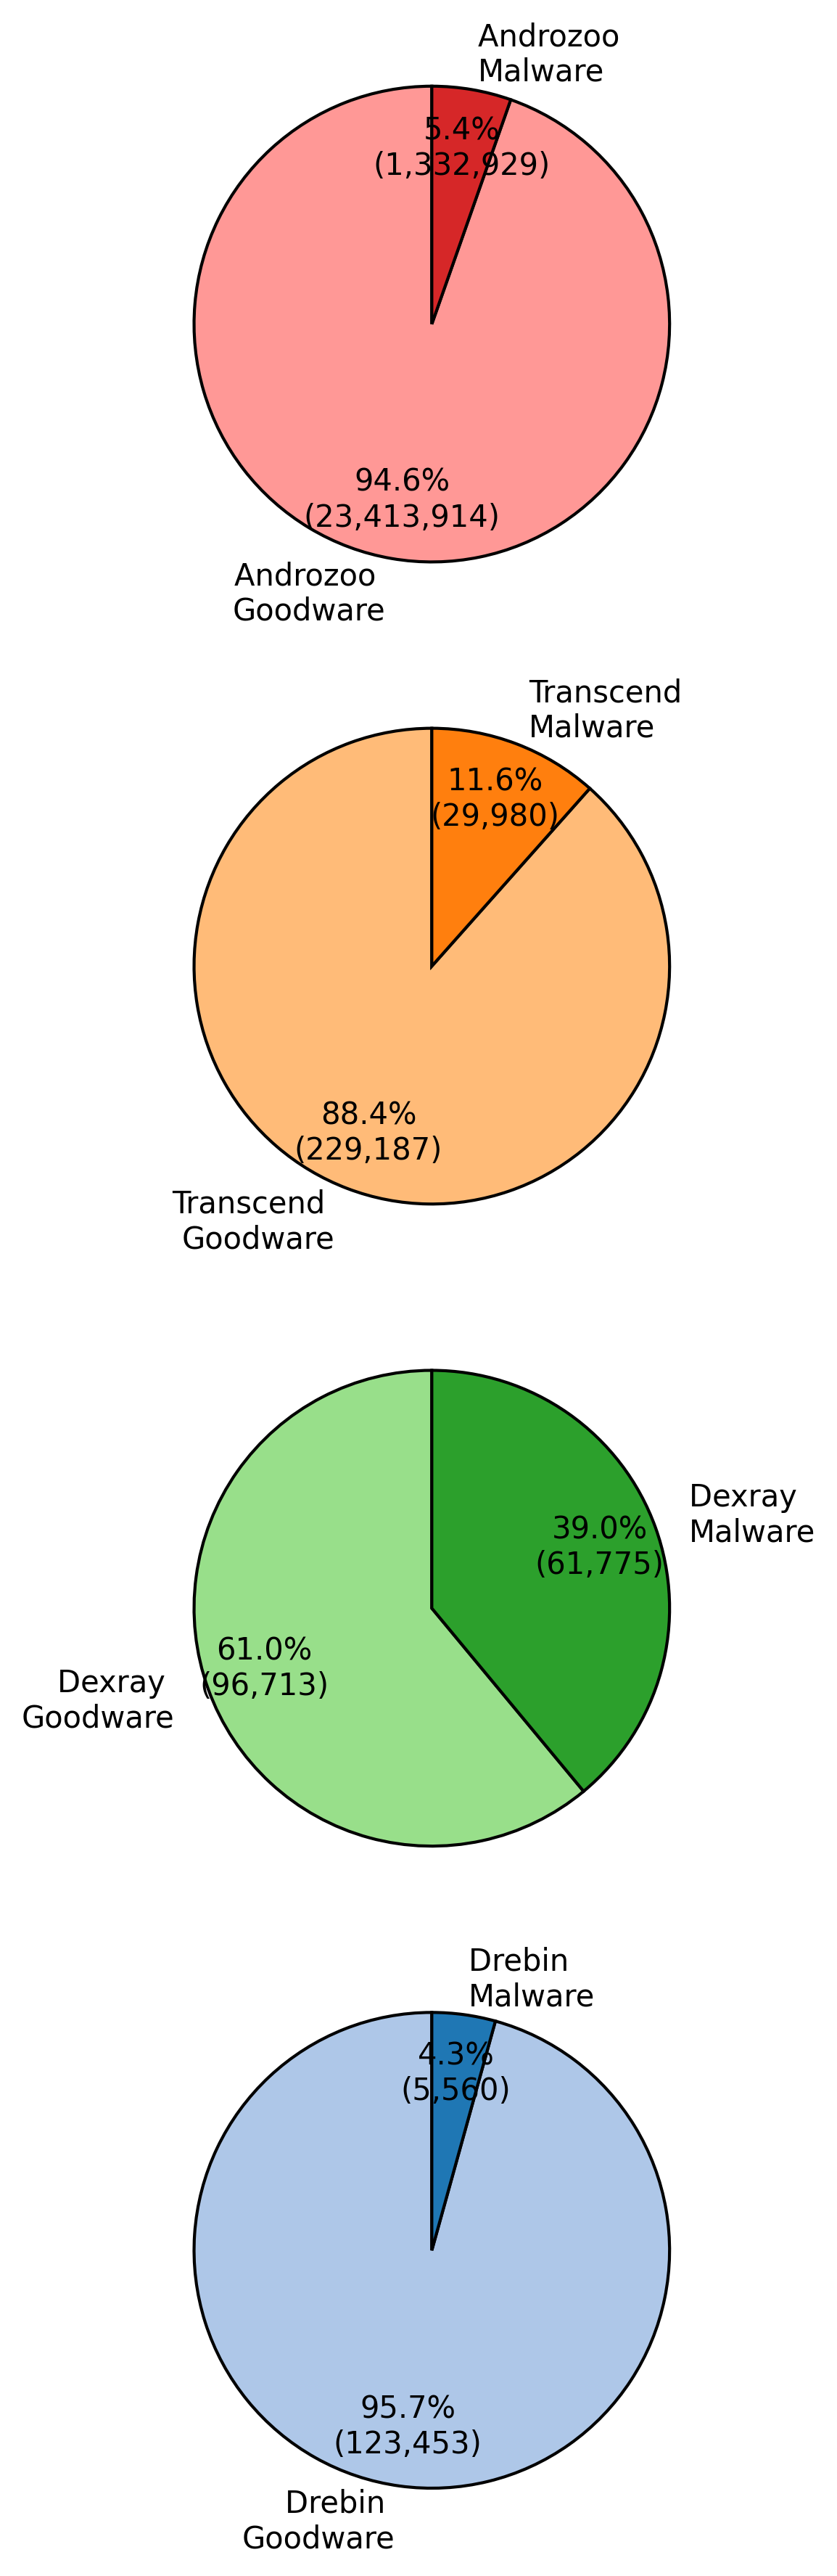
\includegraphics[width=1\marginparwidth]{3_Methodology/malware_goodware_ratios.png}
    \caption{\label{fig:malratios}
    Distribution of malware and goodware samples across datasets shown as pie charts.
    The datasets analyzed are are ordered by size from largest to smallest.
    The number of APKs contained in the Dataset are shown in brackets}
\end{marginfigure}

The evaluation of datasets forms a critical foundation for the success of any machine learning task, especially in security-sensitive applications such as Android malware detection. 
A robust dataset not only enables effective training of models but also ensures generalizability across various scenarios, including concept drift. 
This section outlines the dataset evaluation process undertaken for this research.

The datasets that are evaluated are introduced in subsection \ref{sec:amd}.
The Drebin, Transcending, and DexRay datasets are well-suited for comparison because they are specifically designed to serve as benchmarks for training and evaluating models. 
Each dataset is designed to train specific models and assess their performance effectively. 
Androzoo is notably different because it serves as a large repository for Android APKs rather than a closed dataset specifically designed for training algorithms. 
Additionally, it is continuously updated and expanded by the authors.

When comparing the number of APKs of each dataset, Androzoo has the most APKs with 24,855,480 (as of 25.12.2024 14:47). 
Since it is a repository, it will continue to grow larger.
The biggest of the benchmarking datasets is Transcending, which has 259,230 available APKs. 
This is followed by DexRay with 159,803 APKs, and then Drebin with 129,013 APKs. 
These sizes are significant as they provide varied scales for evaluating model performance. 
In general, larger datasets are better for training and evaluating a model. 
However, this is only true if the dataset size correlates with novelty, meaning it introduces unique and diverse cases. 
For example, a dataset containing applications from various time periods or regions ensures that the model can generalize to unseen scenarios. 
This has been shown by \cite{scalinglaws}, where they demonstrated that the performance of Transformer Decoder Models correlates with the size of the data used to train them.

Figure \ref{fig:malratios} shows the label distribution for each dataset. 
Notably, the Dexray dataset has an unusually high percentage of malware APKs. 
On one hand, this could help the model learn more diverse representations of malicious APKs. 
On the other hand, Arp et al. refer to this as a sampling bias, where "the collected data does not adequately represent the true distribution of the underlying security problem" \cite{dodo}. 
While the actual label distribution is unknown (and likely changes depending on the model's use case), it seems unlikely that 39\% of APKs are generally malware. 
Similarly, the Transcending dataset also has a high malware rate, with over 10\% of its samples being malicious. 
In comparison, Androzoo and Drebin show about 5\% malware APKs in their distributions. 
The Androzoo Malware labels were derived from virustotal\footnote{https://www.virustotal.com/gui/home/upload} by Euphony \cite{androzoo_malware} in 2017, 
which means that they are outdated as newer APKs were not evaluated.

%\vspace*{-2\baselineskip} % Move the figure upwards
\begin{marginfigure}[-50pt] % 't' specifies top placement
    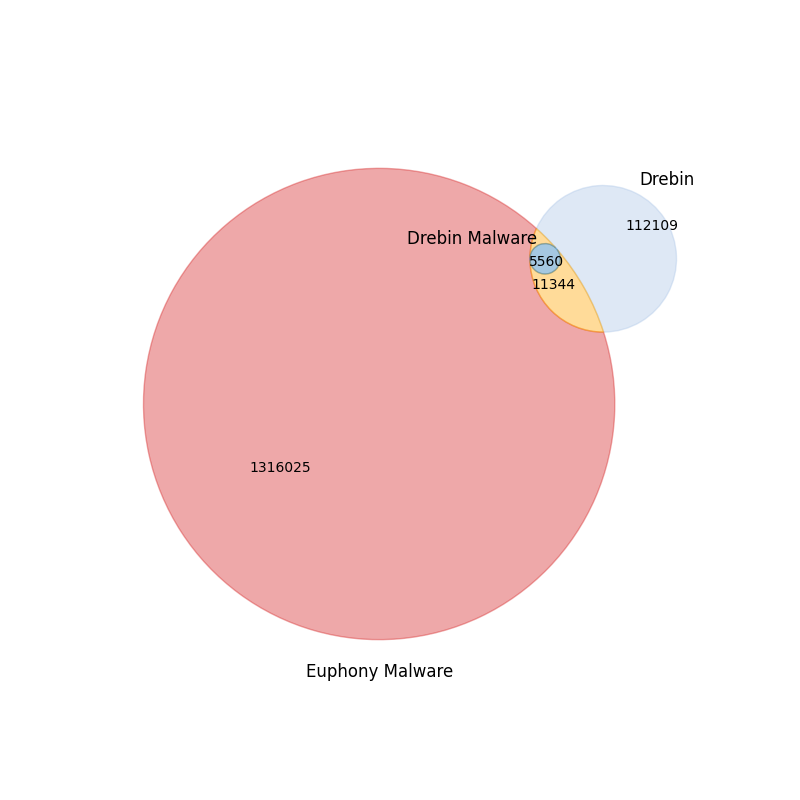
\includegraphics[width=1\marginparwidth]{3_Methodology/euphony_drebin_overlap.png}
    \caption{\label{fig:euphony_drebin_overlap}
    Overlap between the Drebin and Euphony datasets. 
    The light blue circle represents Drebin, where 112,109 APKs are classified as goodware (excluding overlap).
    The red circle represents Euphony, which contains 1,316,025 APKs labeled as malware (excluding overlap). 
    The dark blue circle represent those 5560 APKs, that are considered malware for both Drebin and Euphony.
    The intersection in orange highlights 11,344 APKs classified as goodware by Drebin but as malware by Euphony.}
\end{marginfigure}

One important aspect is that there is no clear definition of malware, which significantly impacts the analysis. 
This lack of a universal definition leads to inconsistencies in classification across datasets, making it challenging to validate labels and draw reliable comparisons. 
Without a standardized framework, each dataset might apply its own criteria.
Each dataset can have different interpretations of what is considered malware, 
often based on criteria such as the presence of specific permissions, API calls, or behaviors flagged by antivirus software. 
For example, one dataset might classify an APK as malware due to aggressive adware practices, while another might only consider code executing malicious payloads. 
These differences make the validation of labels very difficult.
One Example that shows this issue is evident when comparing Drebin with Euphony (Figure: \ref{fig:euphony_drebin_overlap}).
Euphony and Drebin have a common subset, none of the sets is a true subset of the other.
However the APKs labeled as malware by Drebin are a true subset of Euphony.
Additionally Euphony classifies multiple APKs as malware that were classified as goodware by Drebin.
The fact that there are no APKs that are classified as malware by Drebin and Goodware by Euphony shows that Drebin applies a more narrow definition on what is considered malware.
Further Overlaps of different Datasets are visualized in the Appendix (Figure: \ref{fig:dataset_overlap}).



\subsection{Temporal Evaluation}

\begin{figure*}[b]
    \centering
    \begin{minipage}{1.5\textwidth}
        \centering
        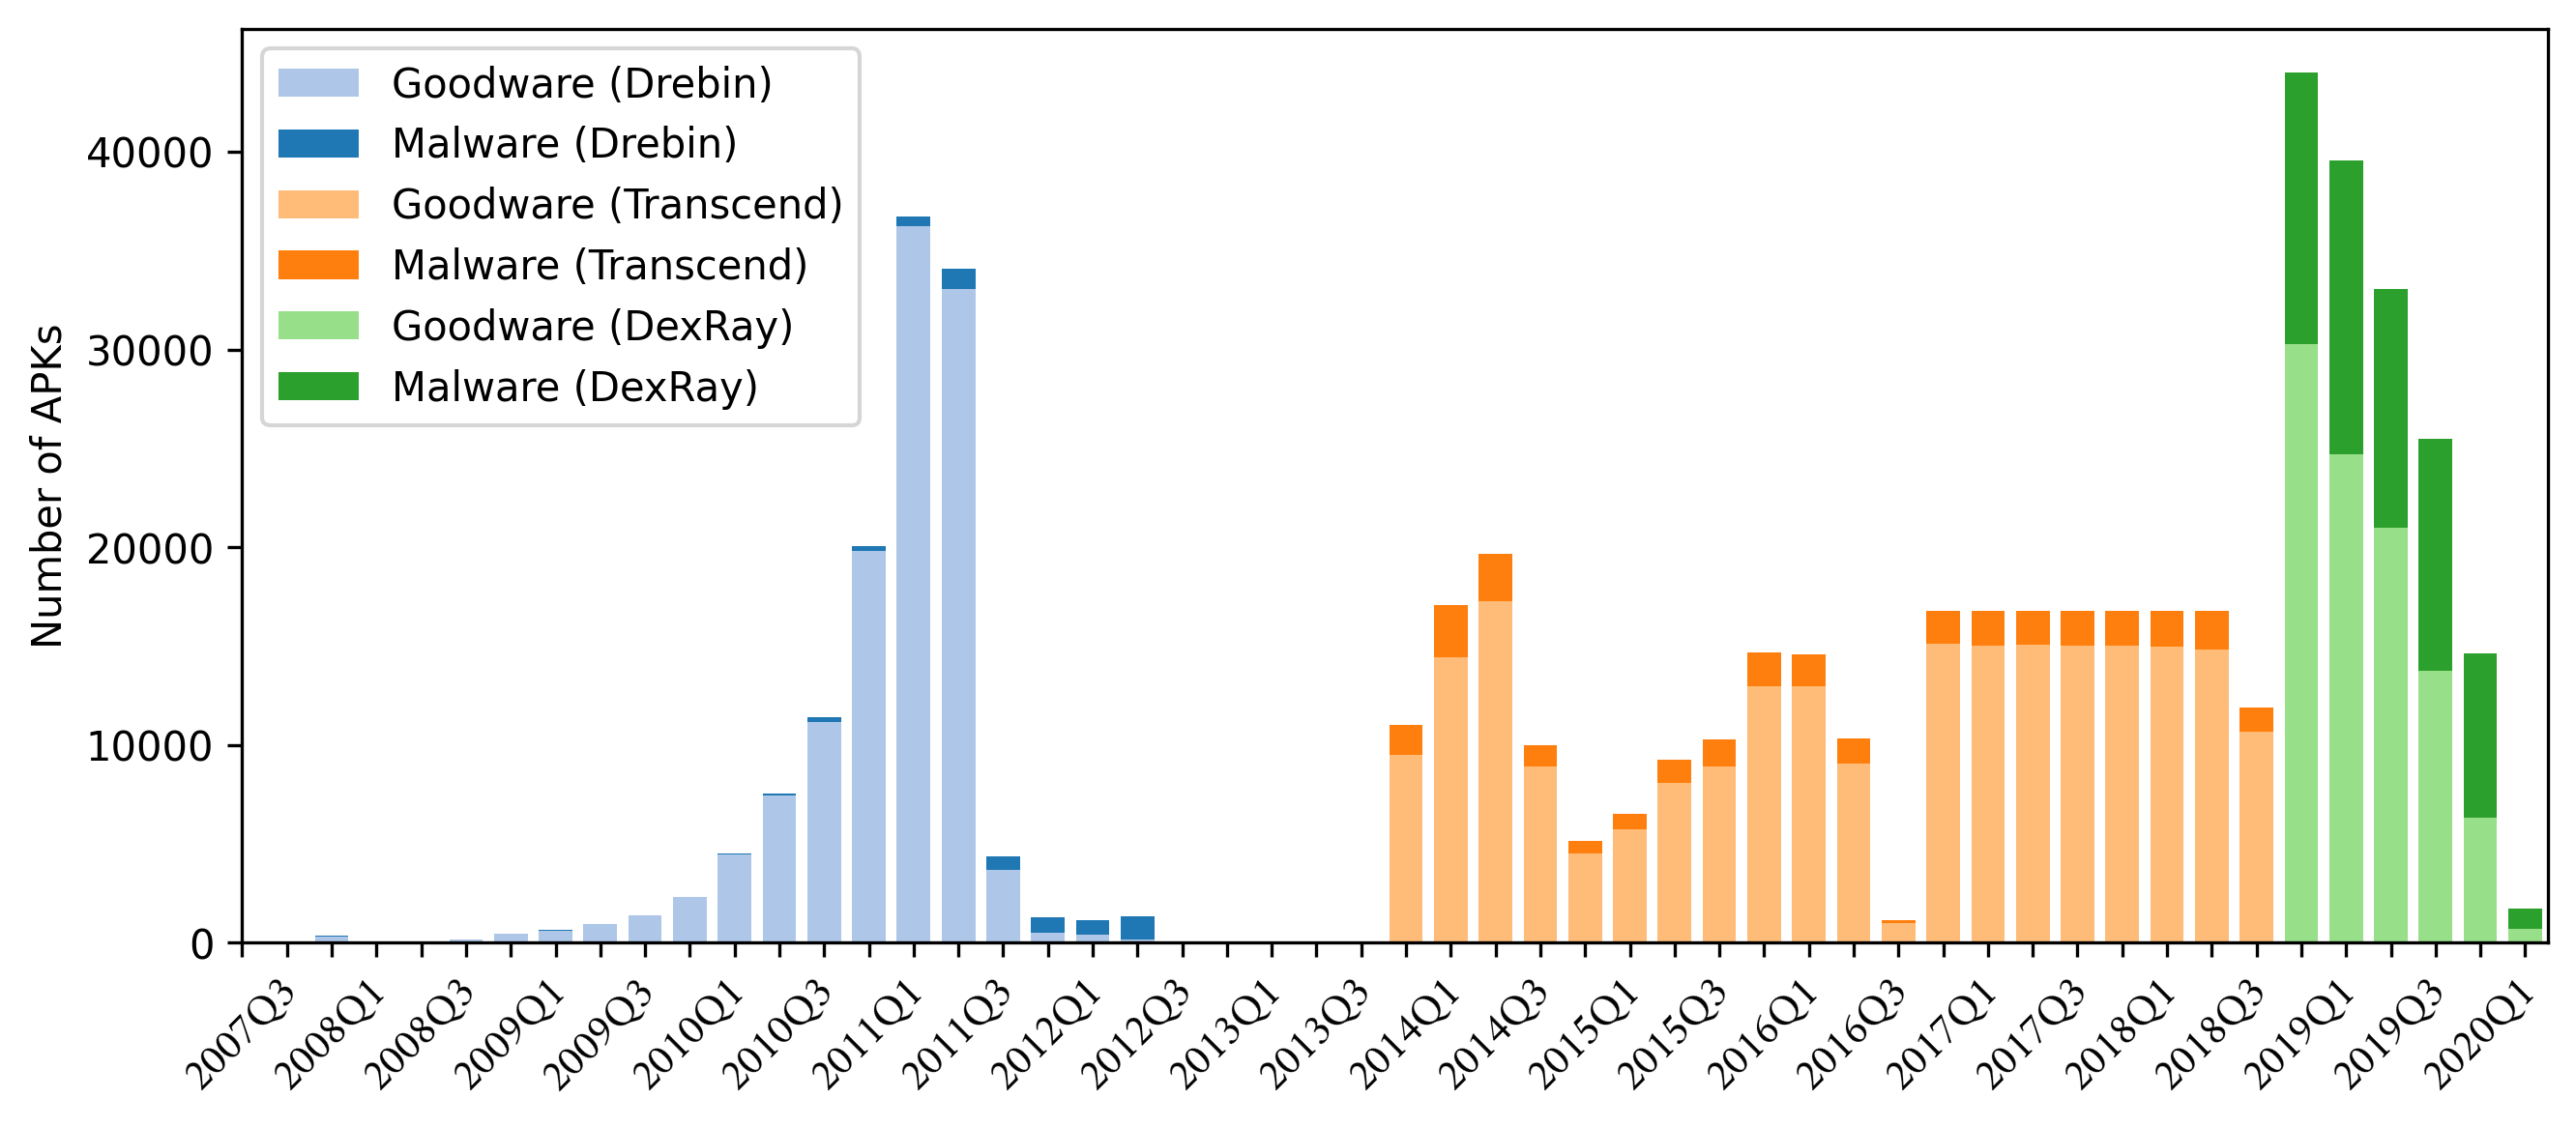
\includegraphics[width=\textwidth]{3_Methodology/dataset_time_distribution.png}
        \captionsetup{width=\textwidth}
        \caption{\label{fig:dataset_time_evaluation}
        Temporal distribution of Android APKs across three datasets (Drebin, Transcend, and DexRay), 
        categorized into goodware and malware.
        The Data is derived from metadata of the classes.dex file of each APK.
        }
    \end{minipage}
\end{figure*}



The temporal evaluation of APKs is often based on metadata of the classes.dex component, as it contains crucial timestamp information reflecting the compilation date of the code. This metadata serves as a reliable indicator of the APK's development period, providing a foundation for chronological analyses.
While this often works (Figure: \ref{fig:dataset_time_evaluation}), it becomes more common that this metainformation is not available. 
This lack of metadata poses challenges for temporal evaluation, as it limits the ability to analyze trends and shifts in malware development over time, 
as seen by the temporal evaluation of the androzoo repository (Figure: \ref{fig:androzoo_temporal})

The distribution of the .dex dates of the three datasets (Figure: \ref{fig:dataset_time_evaluation}) shows that the datasets are in sucession of one another. 
There is no temporal overlap, which explains why there is no APK present in more than one of these datasets (Figure: \ref{fig:dataset_overlap}). 
There is a gap between the third quarters of 2012 and 2013 where neither dataset has samples. 

While the Transcending Dataset seems to be evenly distributed, the other two datasets seem to show varying volumes over time. 
This holds true for the overall volume but also about the evenness of the label distribution. 
Here Drebin and Dexray show unbalanced malware sample behaviour. 
This uneven distribution can affect the generalizability of findings.

% Nochmal Drüberlsesen:::!!! (Extendable)
One Example where concept drift is visible is, that the size of packaged APKs grows with time \ref{fig:dataset_size_evaluation}.
The three datasets show different distributions of APK sizes, where Drebin shows the smallest and DexRay the biggest APKs on average.
The Plot also shows that the labels of all datasets are better distributed by the APK size, compared to the .dex date of the APK.

% Nochmal Drüberlsesen:::!!!
When evaluatig a model regarding the concept drift of malware, the Transcending dataset shows the most potential.
However only considering one dataset limits the generalizability of an approach, so the evaluation on multiple datasets is even better.
One Problem is, that all three datasets only contain APKs where the .dex date is evailable.
The temporal evaluation of Androzoo \ref{fig:androzoo_temporal} showed that this is for most modern APKs not the case.
It follows that each of the datasets are Biased in their selection of of APKs and are therefore not fit for representing the True APK landscape. 



\begin{figure*}[b!]
    \centering
    \begin{minipage}{1.5\textwidth}
        \centering
        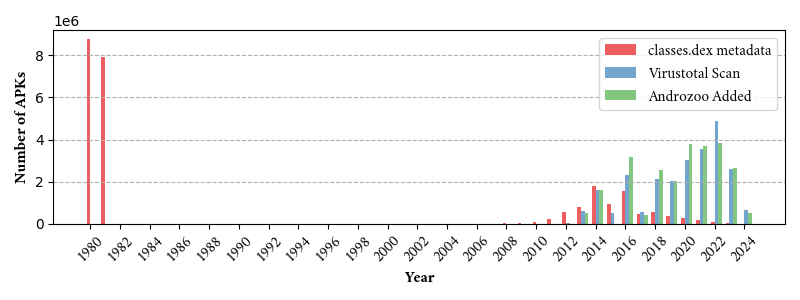
\includegraphics[width=\textwidth]{A_Images/androzoo_temporal.png}
        \captionsetup{width=\textwidth}
        \caption{\label{fig:androzoo_temporal}
        Temporal distribution of APKs based on three key attributes: 
        classes.dex metadata, Virustotal Scan, and Androzoo Added. 
        The red bars (classes.dex metadata) show a large spike in 1980 to 1982, 
        likely due to incorrect or missing metadata values. 
        The blue (year of first scan by virustotal on that APK) and 
        green (year this APK was added to the androzoo repository) bars 
        indicate a consistent increase in APK activity from 2010 onward, 
        peaking around 2020 to 2022, reflecting the growing adoption of Android 
        and corresponding malware collection efforts. 
        The discrepancies between attributes highlight potential issues in 
        dataset metadata accuracy and consistency.
        }
    \end{minipage}
\end{figure*}


\newpage

\subsection{Code Evaluation}

When checkig for Malware, an important representation of an APK is its code.
As the code describes the logic of what the App sould do, it seems logical that if the code is sufficiently evaluated the harmfulness of the APK can be derived.
Especially Transformer models show promise in interpreting the code of an APK as they work very well as Large Language Models.

It follows that not just time distributions of the datasets should be evaluated, but also the distribution of code.
There are two major ways of decompiling an APK into a code representation.
The classes.dex file can either be Decompiled into Java code or into more lower level smali code.

For the decompilation of the APK into Java code, dex2jar\footnote{https://github.com/pxb1988/dex2jar} is first used to decompile the classes.dex file into a JAR file.
The JAR file can then be further decompiled into plain Java code. 
The resulting Java code is on the one hand easier to interpret due to its higher level nature, however the decompiled code is prone to obfuscation that can make it hard to interpret.
One example on how obfuscation can make the logic of the App more complex is by changing the package names, so that it is not possible to see the entry points that are defined in the Manifest file.

There also is an Option to decompile the classes.dex file into Smali code.
Smali is the human readable representation of the Dalvik bytecode that is found in the raw classes.dex file.
Smalie therefore is to Dalvik bytecode, what Assambly is to machine code.
The Smali representation of an APK can be retrieved by using Apktool\footnote{https://apktool.org/} on the classes.dex file.
While the Smali representation is more accurate the the original bytecode and also is more robust to obfuscation, the readability is much harder due to the lower level and nieche nature. 


\begin{figure*}[b!]
    \centering
    \begin{minipage}{1.5\textwidth}
        \centering
        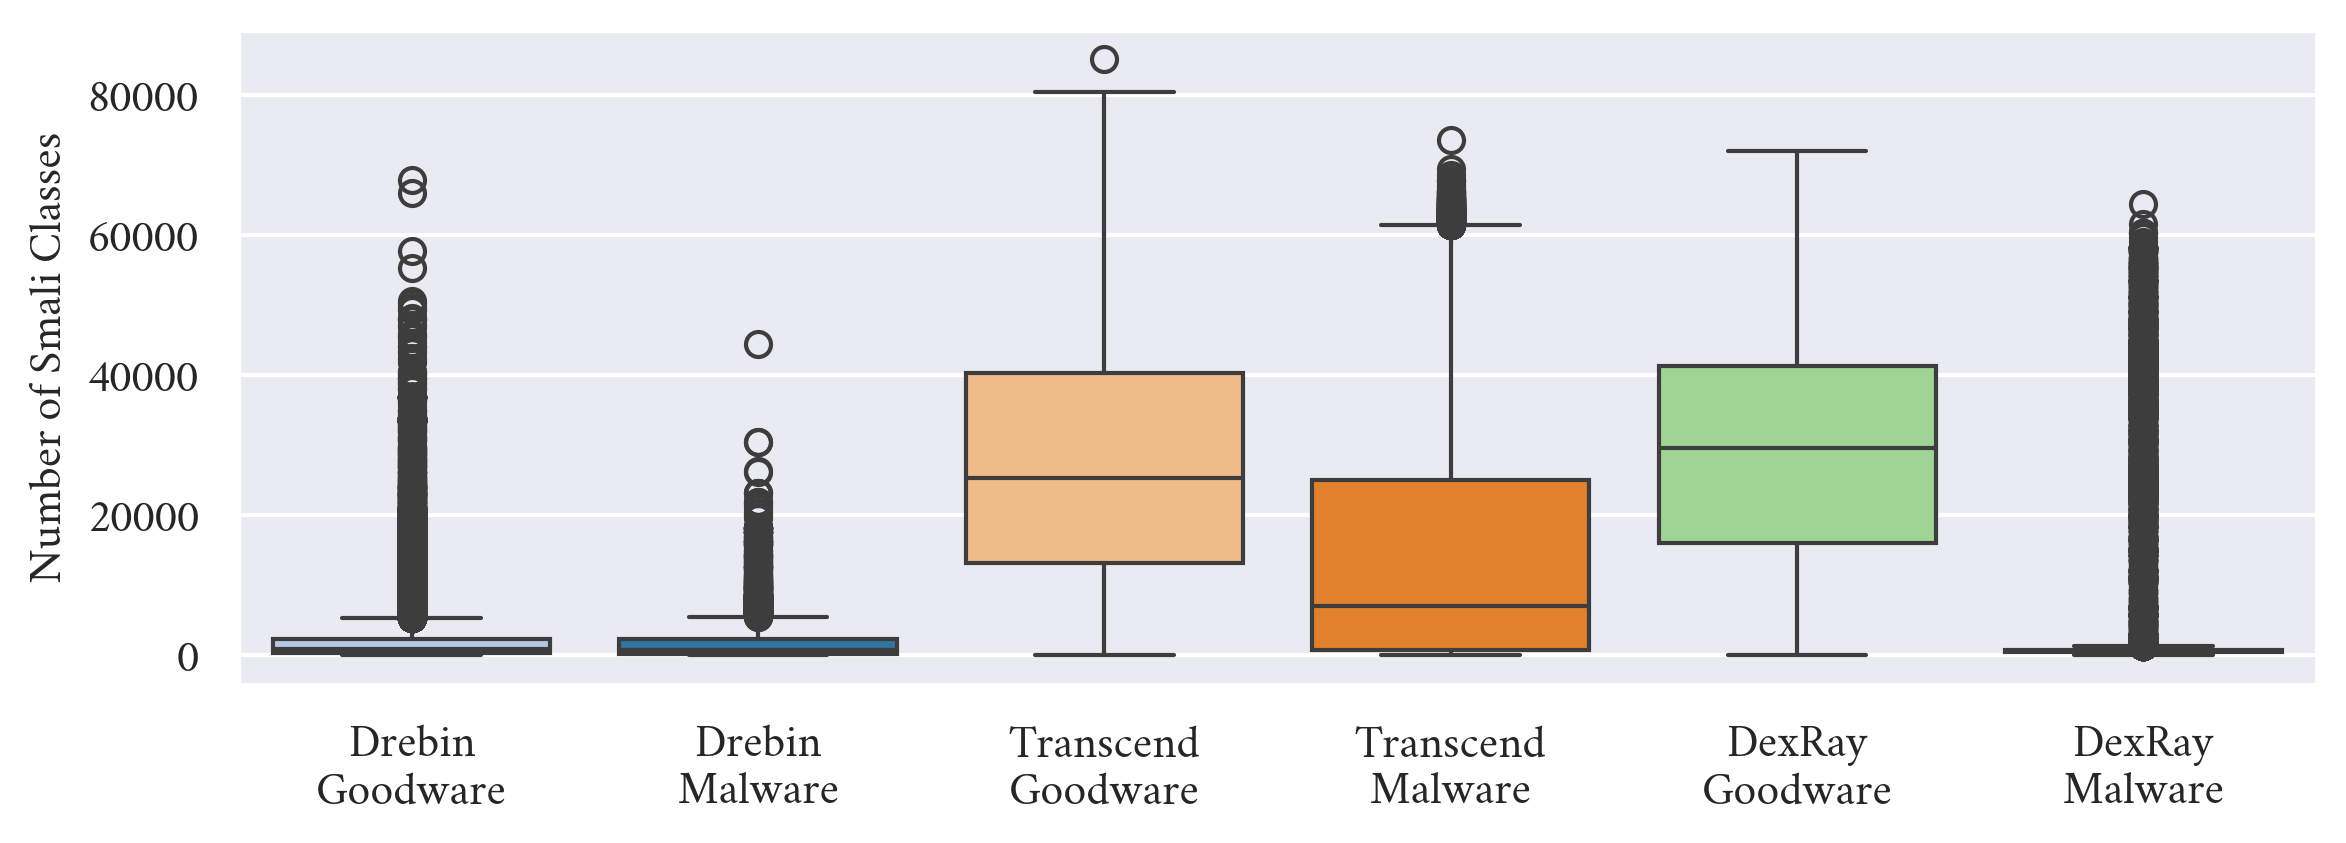
\includegraphics[width=\textwidth]{3_Methodology/smali_class_boxplots.png}
        \captionsetup{width=\textwidth}
        \caption{\label{fig:smali_class_boxplots}
        The boxplot shows the distribution of smali classes in Android apps 
        across the Drebin, Transcend, and DexRay datasets, 
        split into Goodware and Malware. 
        Drebin and Transcend have an similar smali class distribution 
        between Goodware and Malware.
        The DexRay Dataset shows a high inbalance in the number of smali classes 
        between the two labels.
        }
    \end{minipage}
\end{figure*}

\newpage

\begin{margintable}[1\baselineskip] % Move table down by 1 line
    \caption{\label{tab:smali_distribution}Smali Statistics Summary for DexRay, Transcend, and Drebin.}
    \footnotesize
    \begin{tabular}{@{}lccc@{}}
        \toprule
        \tabhead{Label} & \tabhead{Q1} & \tabhead{Median} & \tabhead{Q3} \\
        \midrule
        \multicolumn{4}{l}{\textbf{DexRay}} \\
        Goodware & 16106 & 29546 & 41352 \\
        Malware & 445 & 598 & 817 \\
        \midrule
        \multicolumn{4}{l}{\textbf{Transcend}} \\
        Goodware & 13145 & 25364 & 40372 \\
        Malware & 764 & 7057 & 25015 \\
        \midrule
        \multicolumn{4}{l}{\textbf{Drebin}} \\
        Goodware & 331 & 901 & 2353 \\
        Malware & 173 & 805 & 2316 \\
        \bottomrule
    \end{tabular}
\end{margintable}

As part of the code evaluation of this thesis, 
the same three datasets as i the time evaluation were considered.
Therefore for each APK of the datasets, the classes.dex file was decompiled 
in both an java and an smali representation of the App.
The code representation of an APK is quite complex and only hardly allows 
statistical aalysis.
One approach that was possible is to count the classes of the code representations for each apk,
reducing the compeity from a repository per app to just a number.
Figure \ref{fig:smali_class_boxplots} shows the Boxplots of the distribution 
of smali classes of the apps in the dataset distinguishing 
between the label of the apk.
The Boxplots show, that Drebin has a generally low amount of smali classes 
per APK, wich can be explained by the Apps being 
older \ref{fig:dataset_time_evaluation} and smaller \ref{fig:dataset_size_evaluation} that those of the other datasets.

A second observation that can be made, is that the DexRay Dataset is highly inbalanced.
This is apparent both from the boxplot \ref{fig:smali_class_boxplots} and also the table \ref{tab:smali_distribution},
that quantifies the distribution of smai classes by containing the Q1, Median and Q3 values of each of the Dataset subsets.
When looking further into \ref{tab:smali_distribution} the issue becomes even more apperent. 
Q1, Median and Q3 differ between the labels by a factor of 35-50, this makes any approach that makes label 
predictions based on smali code of that dataset \cite{dexray} \cite{detectbert} questionable.

%\newcolumntype{L}{>{\RaggedRight\arraybackslash}X}
\begin{margintable}[1\baselineskip] % Move table down by 1 line
    \caption{\label{tab:java_distribution}Java Statistics Summary for Drebin, Transcend, and DexRay.}
    \footnotesize
    \begin{tabular}{@{}lccc@{}}
        \toprule
        \tabhead{Label} & \tabhead{Q1} & \tabhead{Median} & \tabhead{Q3} \\
        \midrule
        \multicolumn{4}{l}{\textbf{Drebin}} \\
        Goodware & 19 & 60 & 176 \\
        Malware & 18 & 66 & 224 \\
        \midrule
        \multicolumn{4}{l}{\textbf{Transcend}} \\
        Goodware & 854 & 1800 & 2899 \\
        Malware & 52 & 738 & 2244 \\
        \midrule
        \multicolumn{4}{l}{\textbf{DexRay}} \\
        Goodware & 1035 & 2007 & 3084 \\
        Malware & 7 & 11 & 11 \\
        \bottomrule
    \end{tabular}
\end{margintable}


The Transcending dataset, an class inbalance to a slighter extend that the DexRay dataset.
Especially on Q1 differs by a factor of 17,2 showing that there are relatively more codesparse Malware than Goodware APKs.
When comparing the upper end of the spectrum the inbalance becomes less drastic with an factor of ~3,5 for the median and 1,6 for the Q3.
Drebin shows overall a very good between class balance of smali classes when compared to the other datasets.

The decompilation into java classes paints a similar picture. 
For comparisonthere is in similar structure a table showing the statistical properties of the java class distribution \ref{tab:java_distribution}.
Additionally in the Appendix there is another Boxplot \ref{fig:java_class_boxplots} that has the same structure as figure \ref{fig:smali_class_boxplots}.
When evaluating the java and smali classs values over all datasets a correlation coefficient of 0.92 proofs that they relate a lot.

Table \ref{tab:java_distribution} shows that more than 75\% of the malware APKs have less then 12 Java classes, 
while 75\% have more than 1000 Java Classes.
This make it highly likely that an classifier wil just differentiate 
between the number of classes present and derive the prediction from this.

This leads to the conclusion, that the DexRay dataset is generally insufficient for training a codebased classifier.


\section{Baseline Creation}

\subsection{Naive Approaches}

\subsection{DetectBERT}

\section{Experimntal Setup}

\subsection{Android App Representaion}

\subsection{Model Implementation}

